\documentclass[12pt,a4paper]{article}

%% ---------------------------------------------------------------
%%  PACKAGES
%% ---------------------------------------------------------------
\usepackage{amsmath}
\usepackage{amssymb}
\usepackage{geometry}
\geometry{margin=2.5cm}
\usepackage{booktabs}
\usepackage{xcolor}
\usepackage{hyperref}
\usepackage{listings}
\usepackage{pgfplots}
\pgfplotsset{compat=1.18}
\usepackage{tcolorbox}
\tcbuselibrary{skins, breakable}
\usepackage{enumitem}
\usepackage{fancyhdr}
\usepackage{tikz}
\usepackage{array}
\usepackage{subcaption}

%% ---------------------------------------------------------------
%%  TCOLORBOX ENVIRONMENTS
%% ---------------------------------------------------------------
\newtcolorbox{curiositybox}[1]{colback=yellow!10, colframe=orange!80!black, fonttitle=\bfseries, title=#1, breakable}
\newtcolorbox{infobox}[1]{colback=blue!5, colframe=blue!60!black, fonttitle=\bfseries, title=#1, breakable}
\newtcolorbox{mistakebox}[1]{colback=red!5, colframe=red!60!black, fonttitle=\bfseries, title=#1, breakable}
\newtcolorbox{learnbox}[1]{colback=green!5, colframe=green!60!black, fonttitle=\bfseries, title=#1, breakable}

%% ---------------------------------------------------------------
%%  LISTINGS — PYTHON
%% ---------------------------------------------------------------
\lstset{language=Python, basicstyle=\ttfamily\small, keywordstyle=\color{blue},
        commentstyle=\color{gray}, stringstyle=\color{orange},
        showstringspaces=false, numbers=left, numberstyle=\tiny,
        breaklines=true, frame=single}

%% ---------------------------------------------------------------
%%  FANCYHDR
%% ---------------------------------------------------------------
\pagestyle{fancy}
\fancyhf{}
\lhead{Topic 03: Even and Odd Functions}
\rhead{Unit V --- Fourier Series \& Transforms}
\cfoot{\thepage}

%% ---------------------------------------------------------------
%%  TITLE
%% ---------------------------------------------------------------
\title{Topic 03: Fourier Series of Even and Odd Functions \\
       \large Unit V --- Fourier Series \& Fourier Transforms}
\author{23A54201 --- Mathematics IV (Transform Techniques) \\
        JNTUA College of Engineering (Autonomous)}
\date{}

%% ===============================================================
\begin{document}
%% ===============================================================

\maketitle
\tableofcontents
\newpage

%% ---------------------------------------------------------------
\section{Opening Hook}
%% ---------------------------------------------------------------

\begin{curiositybox}{Hook}
When you compute the Fourier series of $f(x)=x^2$ on $(-\pi,\pi)$, you spend 15 minutes
integrating to find $b_n$ --- and they ALL turn out to be zero. Every single one. Was that
time wasted? Yes, completely --- and it didn't have to be. If you had noticed that $x^2$ is
an EVEN function (symmetric about the $y$-axis), you could have declared $b_n=0$ in three
seconds without touching a single integral. That's the power of symmetry.
\end{curiositybox}

%% ---------------------------------------------------------------
\section{Why This Topic Exists}
%% ---------------------------------------------------------------

Before we begin, here is the honest answer to why you are reading this: recognising even or
odd symmetry \emph{before} integrating can cut your computation effort in half and immediately
eliminate entire sets of Fourier coefficients. In an examination with limited time, declaring
``this function is even, therefore $b_n = 0$ for all $n$'' in a single line is far more
powerful than grinding through every integral separately. Engineers also encounter even and odd
functions constantly --- vibration modes, signal waveforms, and heat distributions all obey
these symmetries.

\medskip

The table below shows what happens when you skip the symmetry check versus when you exploit it.

\begin{center}
\begin{tabular}{@{}ll@{}}
\toprule
\textbf{Mistake / Shortcut Skipped} & \textbf{Consequence} \\
\midrule
Computing all coefficients without checking symmetry &
    Wasting exam time on integrals that are provably zero \\
Confusing even/odd function definition &
    Wrongly declaring all $a_n = 0$ for an even function \\
Forgetting symmetry only applies to symmetric intervals &
    Applying even/odd shortcuts on non-symmetric domains \\
\bottomrule
\end{tabular}
\end{center}

\begin{learnbox}{Takeaway}
Always test a function for even/odd symmetry \emph{first}. It costs ten seconds and can save
fifteen minutes of integration.
\end{learnbox}

%% ---------------------------------------------------------------
\section{You Already Know This (Intuition First)}
%% ---------------------------------------------------------------

Think of a see-saw perfectly balanced at its centre. An \textbf{even function} behaves exactly
like that perfectly balanced see-saw: the left half of its graph is a mirror image of the right
half. Because of this perfect symmetry, all the Fourier ``weight'' lies on the cosine side
(cosines are themselves even) and none on the sine side (sines are odd --- they would break the
balance).

An \textbf{odd function} is the opposite: tip the see-saw so the left side goes up when the
right side goes down. The graph has a 180\textdegree\ rotational symmetry about the origin.
All its Fourier weight sits on the sine side. When you multiply an odd function by a cosine
(even), you get an odd product, and integrating an odd function over a symmetric interval
$(-\pi, \pi)$ gives exactly zero --- every time, automatically.

There is nothing magical here: it is pure geometry. Once you \emph{see} the symmetry of the
graph, you know which coefficients vanish before touching a single integral.

%% ---------------------------------------------------------------
\section{Definitions: Even and Odd Functions}
%% ---------------------------------------------------------------

\begin{infobox}{Formal Definitions and Key Integral Properties}
\textbf{Even function:} A function $f$ is called \emph{even} if
\[
  f(-x) = f(x) \quad \text{for all } x \text{ in its domain.}
\]
Its graph is symmetric about the $y$-axis.
\textbf{Examples:} $\cos(x)$, $x^2$, $|x|$, any constant.

\medskip

\textbf{Odd function:} A function $f$ is called \emph{odd} if
\[
  f(-x) = -f(x) \quad \text{for all } x \text{ in its domain.}
\]
Its graph has 180\textdegree\ rotational symmetry about the origin.
\textbf{Examples:} $\sin(x)$, $x$, $x^3$.

\medskip

\textbf{Key integral properties on a symmetric interval $[-a, a]$:}
\[
  \int_{-a}^{a} g(x)\,dx = 0 \quad \text{if } g \text{ is odd,}
\]
\[
  \int_{-a}^{a} g(x)\,dx = 2\int_{0}^{a} g(x)\,dx \quad \text{if } g \text{ is even.}
\]
These two facts are the entire engine behind the even/odd Fourier shortcut.
\end{infobox}

\subsection*{Graphs of an Even and an Odd Function}

The figure below shows $f(x)=x^2$ (even, symmetric about the $y$-axis) and $g(x)=x$
(odd, antisymmetric about the origin) plotted on $[-\pi, \pi]$.

\begin{figure}[h]
\centering
\begin{subfigure}[b]{0.48\textwidth}
\centering
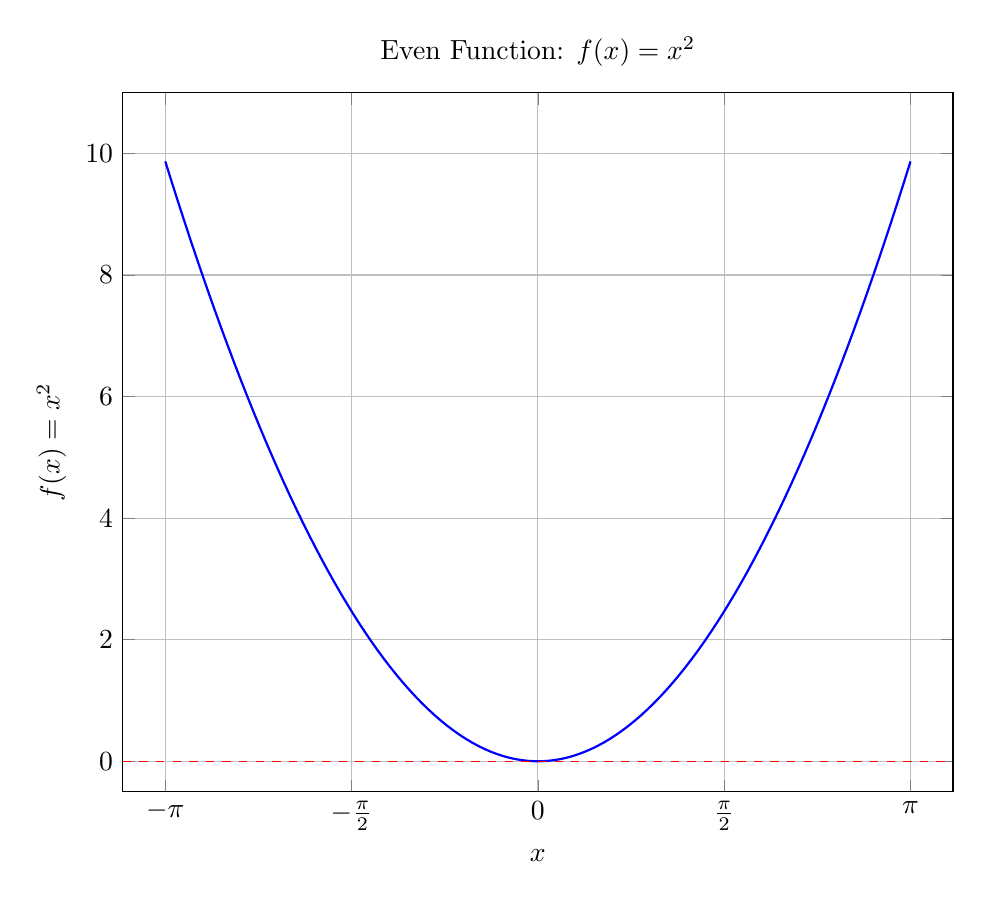
\begin{tikzpicture}
\begin{axis}[
    xlabel={$x$}, ylabel={$f(x) = x^2$},
    xmin=-3.5, xmax=3.5,
    ymin=-0.5, ymax=11,
    grid=major,
    width=\textwidth,
    title={Even Function: $f(x)=x^2$},
    xtick={-3.14159, -1.5708, 0, 1.5708, 3.14159},
    xticklabels={$-\pi$, $-\tfrac{\pi}{2}$, $0$, $\tfrac{\pi}{2}$, $\pi$}
]
\addplot[blue, thick, domain=-3.14159:3.14159, samples=120] {x^2};
\addplot[dashed, red, domain=-3.5:3.5] {0};
\end{axis}
\end{tikzpicture}
\caption{$f(x)=x^2$: symmetric about the $y$-axis (even)}
\end{subfigure}
\hfill
\begin{subfigure}[b]{0.48\textwidth}
\centering
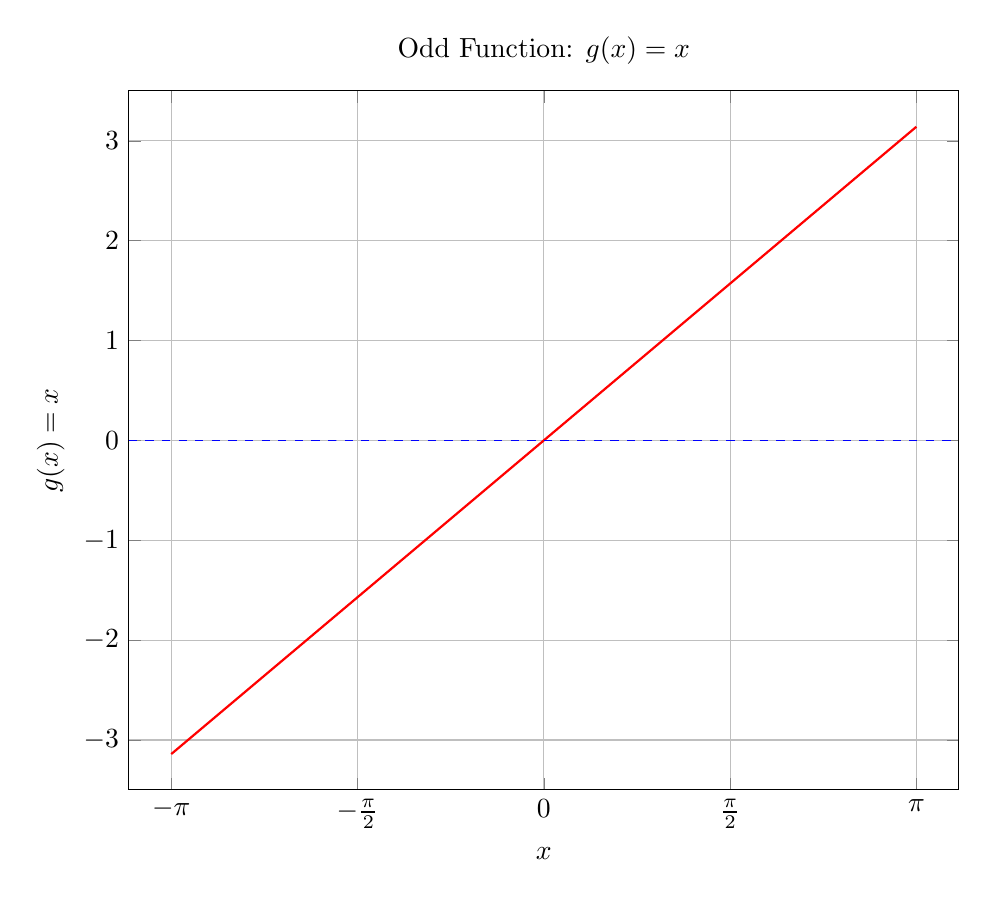
\begin{tikzpicture}
\begin{axis}[
    xlabel={$x$}, ylabel={$g(x) = x$},
    xmin=-3.5, xmax=3.5,
    ymin=-3.5, ymax=3.5,
    grid=major,
    width=\textwidth,
    title={Odd Function: $g(x)=x$},
    xtick={-3.14159, -1.5708, 0, 1.5708, 3.14159},
    xticklabels={$-\pi$, $-\tfrac{\pi}{2}$, $0$, $\tfrac{\pi}{2}$, $\pi$}
]
\addplot[red, thick, domain=-3.14159:3.14159, samples=80] {x};
\addplot[dashed, blue, domain=-3.5:3.5] {0};
\end{axis}
\end{tikzpicture}
\caption{$g(x)=x$: rotational symmetry about origin (odd)}
\end{subfigure}
\caption{Side-by-side comparison of an even and an odd function on $[-\pi,\pi]$.}
\end{figure}

%% ---------------------------------------------------------------
\section{Fourier Series of Even Functions}
%% ---------------------------------------------------------------

\begin{infobox}{Derivation: Fourier Series of an Even Function on $(-\pi,\pi)$}
Recall the general Fourier coefficients on $(-\pi, \pi)$:
\[
  a_0 = \frac{1}{\pi}\int_{-\pi}^{\pi} f(x)\,dx, \quad
  a_n = \frac{1}{\pi}\int_{-\pi}^{\pi} f(x)\cos(nx)\,dx, \quad
  b_n = \frac{1}{\pi}\int_{-\pi}^{\pi} f(x)\sin(nx)\,dx.
\]

\textbf{Step 1 --- $b_n$ vanishes:}
If $f(x)$ is even, then $f(x)\sin(nx)$ is the product of an \emph{even} function and an
\emph{odd} function ($\sin(nx)$ is odd). Even $\times$ Odd $=$ Odd. The integral of an odd
function over the symmetric interval $(-\pi,\pi)$ is zero:
\[
  b_n = \frac{1}{\pi}\int_{-\pi}^{\pi} \underbrace{f(x)\sin(nx)}_{\text{odd}} \,dx = 0
  \quad \text{for all } n \geq 1.
\]

\textbf{Step 2 --- Simplify $a_0$:}
$f(x)$ is even, so its integral over $(-\pi,\pi)$ is twice the integral over $(0,\pi)$:
\[
  a_0 = \frac{1}{\pi}\cdot 2\int_{0}^{\pi} f(x)\,dx
      = \frac{2}{\pi}\int_{0}^{\pi} f(x)\,dx.
\]

\textbf{Step 3 --- Simplify $a_n$:}
$f(x)\cos(nx)$ is even $\times$ even $=$ even, so again we halve the interval:
\[
  a_n = \frac{1}{\pi}\cdot 2\int_{0}^{\pi} f(x)\cos(nx)\,dx
      = \frac{2}{\pi}\int_{0}^{\pi} f(x)\cos(nx)\,dx.
\]

\textbf{Conclusion:} The Fourier series of an even function on $(-\pi,\pi)$ is a
\textbf{pure cosine series}:
\[
  \boxed{f(x) = \frac{a_0}{2} + \sum_{n=1}^{\infty} a_n\cos(nx),}
  \qquad
  a_0 = \frac{2}{\pi}\int_{0}^{\pi} f(x)\,dx, \quad
  a_n = \frac{2}{\pi}\int_{0}^{\pi} f(x)\cos(nx)\,dx.
\]
No sine terms appear.
\end{infobox}

%% ---------------------------------------------------------------
\section{Fourier Series of Odd Functions}
%% ---------------------------------------------------------------

\begin{infobox}{Derivation: Fourier Series of an Odd Function on $(-\pi,\pi)$}
\textbf{Step 1 --- $a_0$ vanishes:}
If $f(x)$ is odd, then $f(x)$ itself is odd. The integral of an odd function over a symmetric
interval is zero:
\[
  a_0 = \frac{1}{\pi}\int_{-\pi}^{\pi} \underbrace{f(x)}_{\text{odd}} \,dx = 0.
\]

\textbf{Step 2 --- $a_n$ vanishes:}
$f(x)\cos(nx)$ is odd $\times$ even $=$ odd. Therefore:
\[
  a_n = \frac{1}{\pi}\int_{-\pi}^{\pi} \underbrace{f(x)\cos(nx)}_{\text{odd}} \,dx = 0
  \quad \text{for all } n \geq 1.
\]

\textbf{Step 3 --- Simplify $b_n$:}
$f(x)\sin(nx)$ is odd $\times$ odd $=$ even. So:
\[
  b_n = \frac{1}{\pi}\cdot 2\int_{0}^{\pi} f(x)\sin(nx)\,dx
      = \frac{2}{\pi}\int_{0}^{\pi} f(x)\sin(nx)\,dx.
\]

\textbf{Conclusion:} The Fourier series of an odd function on $(-\pi,\pi)$ is a
\textbf{pure sine series}:
\[
  \boxed{f(x) = \sum_{n=1}^{\infty} b_n\sin(nx),}
  \qquad
  b_n = \frac{2}{\pi}\int_{0}^{\pi} f(x)\sin(nx)\,dx.
\]
No constant term and no cosine terms appear.
\end{infobox}

%% ---------------------------------------------------------------
\section{Quick-Identification Table}
%% ---------------------------------------------------------------

Use the table below as a quick reference during problem solving.

\begin{center}
\begin{tabular}{@{}llll@{}}
\toprule
\textbf{Function} & \textbf{Even / Odd / Neither} &
\textbf{Coefficients That Vanish} & \textbf{Series Type} \\
\midrule
$x$             & Odd     & $a_0, a_n$        & Pure sine \\
$x^2$           & Even    & $b_n$             & Pure cosine \\
$x^3$           & Odd     & $a_0, a_n$        & Pure sine \\
$|x|$           & Even    & $b_n$             & Pure cosine \\
$\cos(x)$       & Even    & $b_n$             & Pure cosine \\
$\sin(x)$       & Odd     & $a_0, a_n$        & Pure sine \\
$e^x$           & Neither & None vanish automatically & Full series \\
Square wave (symmetric) & Even & $b_n$         & Pure cosine \\
\bottomrule
\end{tabular}
\end{center}

%% ---------------------------------------------------------------
\section{Products of Even and Odd Functions}
%% ---------------------------------------------------------------

\begin{infobox}{Product Rules for Even and Odd Functions}
The parity of a product follows the same rules as multiplication of signs:

\medskip
\begin{center}
\begin{tabular}{@{}lll@{}}
\toprule
\textbf{Factor 1} & \textbf{Factor 2} & \textbf{Product} \\
\midrule
Even & Even & Even \\
Odd  & Odd  & Even \\
Even & Odd  & Odd  \\
Odd  & Even & Odd  \\
\bottomrule
\end{tabular}
\end{center}

\medskip
\textbf{Why does this matter?} Fourier coefficients are integrals of the form
$\int_{-\pi}^{\pi} f(x)\,g(x)\,dx$, where $g(x)$ is either $\cos(nx)$ (even) or $\sin(nx)$
(odd). The product rules above tell you immediately whether the integrand is even or odd ---
and hence whether the integral is zero (odd integrand) or can be halved to $(0,\pi)$
(even integrand). This is the complete theoretical justification for the entire even/odd
shortcut.
\end{infobox}

%% ---------------------------------------------------------------
\section{Worked Examples}
%% ---------------------------------------------------------------

%% --- Example 1 ------------------------------------------------
\begin{infobox}{Example 1: Fourier Series of $f(x) = x^2$ on $(-\pi, \pi)$}
\textbf{Step 1 --- Identify symmetry.}
Check: $f(-x) = (-x)^2 = x^2 = f(x)$. So $f(x) = x^2$ is \textbf{even}.
Declare immediately: $b_n = 0$ for all $n \geq 1$.

\medskip
\textbf{Step 2 --- Compute $a_0$.}
\[
  a_0 = \frac{2}{\pi}\int_{0}^{\pi} x^2\,dx
      = \frac{2}{\pi}\left[\frac{x^3}{3}\right]_{0}^{\pi}
      = \frac{2}{\pi}\cdot\frac{\pi^3}{3}
      = \frac{2\pi^2}{3}.
\]

\textbf{Step 3 --- Compute $a_n$.}
\[
  a_n = \frac{2}{\pi}\int_{0}^{\pi} x^2\cos(nx)\,dx.
\]
Integrate by parts twice. Let $u = x^2$, $dv = \cos(nx)\,dx$, so $du = 2x\,dx$,
$v = \frac{\sin(nx)}{n}$:
\[
  \int_{0}^{\pi} x^2\cos(nx)\,dx
  = \left[\frac{x^2\sin(nx)}{n}\right]_{0}^{\pi}
    - \frac{2}{n}\int_{0}^{\pi} x\sin(nx)\,dx.
\]
The first term vanishes because $\sin(n\pi) = 0$. Now for $\int_{0}^{\pi} x\sin(nx)\,dx$,
let $u = x$, $dv = \sin(nx)\,dx$, so $du = dx$, $v = -\frac{\cos(nx)}{n}$:
\[
  \int_{0}^{\pi} x\sin(nx)\,dx
  = \left[-\frac{x\cos(nx)}{n}\right]_{0}^{\pi}
    + \frac{1}{n}\int_{0}^{\pi}\cos(nx)\,dx
  = -\frac{\pi\cos(n\pi)}{n}
    + \frac{1}{n}\left[\frac{\sin(nx)}{n}\right]_{0}^{\pi}.
\]
The boundary term of the last integral is zero because $\sin(n\pi) = 0$. So:
\[
  \int_{0}^{\pi} x\sin(nx)\,dx = -\frac{\pi(-1)^n}{n} = \frac{(-1)^{n+1}\pi}{n}.
\]
Substituting back:
\[
  \int_{0}^{\pi} x^2\cos(nx)\,dx
  = -\frac{2}{n}\cdot\frac{(-1)^{n+1}\pi}{n}
  = \frac{2(-1)^n\pi}{n^2}.
\]
Therefore:
\[
  a_n = \frac{2}{\pi}\cdot\frac{2(-1)^n\pi}{n^2} = \frac{4(-1)^n}{n^2}.
\]

\textbf{Step 4 --- Write the Fourier series.}
\[
  x^2 = \frac{\pi^2}{3} + \sum_{n=1}^{\infty}\frac{4(-1)^n}{n^2}\cos(nx)
       = \frac{\pi^2}{3} - 4\cos(x) + \cos(2x) - \frac{4}{9}\cos(3x) + \cdots
\]

\textbf{Step 5 --- Derive the famous result $\displaystyle\sum_{n=1}^{\infty}\frac{1}{n^2} = \frac{\pi^2}{6}$.}
Set $x = \pi$ (a point of continuity at the boundary; by Dirichlet, the series converges to
$f(\pi) = \pi^2$):
\[
  \pi^2 = \frac{\pi^2}{3} + \sum_{n=1}^{\infty}\frac{4(-1)^n}{n^2}(-1)^n
         = \frac{\pi^2}{3} + 4\sum_{n=1}^{\infty}\frac{1}{n^2}.
\]
So:
\[
  \pi^2 - \frac{\pi^2}{3} = 4\sum_{n=1}^{\infty}\frac{1}{n^2}
  \implies \frac{2\pi^2}{3} = 4\sum_{n=1}^{\infty}\frac{1}{n^2}
  \implies \sum_{n=1}^{\infty}\frac{1}{n^2} = \frac{\pi^2}{6}. \qquad\checkmark
\]
\end{infobox}

\begin{learnbox}{What Did We Learn? (Example 1)}
For $f(x) = x^2$: recognising it is even eliminates all $b_n$ integrals immediately.
The resulting pure cosine series can be evaluated at a specific point ($x = \pi$) to derive
the celebrated result $\sum 1/n^2 = \pi^2/6$. Symmetry is not just a computational shortcut
--- it unlocks deeper mathematical identities.
\end{learnbox}

%% --- Example 2 ------------------------------------------------
\begin{infobox}{Example 2: Fourier Series of $f(x) = x$ on $(-\pi, \pi)$}
\textbf{Step 1 --- Identify symmetry.}
Check: $f(-x) = -x = -f(x)$. So $f(x) = x$ is \textbf{odd}.
Declare immediately: $a_0 = 0$ and $a_n = 0$ for all $n \geq 1$.

\medskip
\textbf{Step 2 --- Compute $b_n$.}
\[
  b_n = \frac{2}{\pi}\int_{0}^{\pi} x\sin(nx)\,dx.
\]
Integrate by parts: $u = x$, $dv = \sin(nx)\,dx$, $du = dx$, $v = -\cos(nx)/n$:
\[
  \int_{0}^{\pi} x\sin(nx)\,dx
  = \left[-\frac{x\cos(nx)}{n}\right]_{0}^{\pi}
    + \frac{1}{n}\int_{0}^{\pi}\cos(nx)\,dx
  = -\frac{\pi\cos(n\pi)}{n} + \frac{\sin(n\pi)}{n^2}.
\]
Since $\sin(n\pi) = 0$ and $\cos(n\pi) = (-1)^n$:
\[
  \int_{0}^{\pi} x\sin(nx)\,dx = -\frac{\pi(-1)^n}{n} = \frac{(-1)^{n+1}\pi}{n}.
\]
Therefore:
\[
  b_n = \frac{2}{\pi}\cdot\frac{(-1)^{n+1}\pi}{n} = \frac{2(-1)^{n+1}}{n}.
\]

\textbf{Step 3 --- Write the Fourier series.}
\[
  x = 2\sum_{n=1}^{\infty}\frac{(-1)^{n+1}}{n}\sin(nx)
    = 2\left(\sin(x) - \frac{\sin(2x)}{2} + \frac{\sin(3x)}{3} - \cdots\right).
\]
\end{infobox}

\begin{learnbox}{What Did We Learn? (Example 2)}
$f(x) = x$ is odd, so its entire Fourier series consists solely of sine terms. Setting $x =
\pi/2$ in this result and using the known values of $\sin(n\pi/2)$ yields the Leibniz formula
$\pi/4 = 1 - 1/3 + 1/5 - \cdots$. Odd functions and sine series are inseparable partners.
\end{learnbox}

%% --- Example 3 ------------------------------------------------
\begin{infobox}{Example 3: Fourier Series of $f(x) = x + x^2$ on $(-\pi, \pi)$}
\textbf{Step 1 --- Check symmetry.}
Test even: $f(-x) = -x + x^2$. Is this equal to $f(x) = x + x^2$? No.
Test odd: Is $f(-x) = -f(x) = -x - x^2$? No.
Therefore $f(x) = x + x^2$ is \textbf{neither even nor odd}.

\medskip
\textbf{Step 2 --- Decompose into even and odd parts.}
Every function can be split uniquely as $f(x) = f_e(x) + f_o(x)$, where:
\[
  f_e(x) = \frac{f(x) + f(-x)}{2}, \qquad
  f_o(x) = \frac{f(x) - f(-x)}{2}.
\]
With $f(x) = x + x^2$ and $f(-x) = -x + x^2$:
\[
  f_e(x) = \frac{(x+x^2)+(-x+x^2)}{2} = \frac{2x^2}{2} = x^2,
\]
\[
  f_o(x) = \frac{(x+x^2)-(-x+x^2)}{2} = \frac{2x}{2} = x.
\]
So $x + x^2 = x^2 + x$ --- the even part is $x^2$ and the odd part is $x$, which are
precisely the functions from Examples 1 and 2.

\medskip
\textbf{Step 3 --- Write the full Fourier series by linearity.}
\[
  x + x^2 = \frac{\pi^2}{3} + \sum_{n=1}^{\infty}\frac{4(-1)^n}{n^2}\cos(nx)
             + 2\sum_{n=1}^{\infty}\frac{(-1)^{n+1}}{n}\sin(nx).
\]
This is a mixed series (both cosine and sine terms), as expected for a function that is
neither even nor odd.
\end{infobox}

\begin{learnbox}{What Did We Learn? (Example 3)}
Any function can be split into its even part $f_e = (f(x)+f(-x))/2$ and odd part
$f_o = (f(x)-f(-x))/2$. The Fourier series then follows by superposition. This decomposition
is the general strategy when a function has no obvious symmetry.
\end{learnbox}

%% ---------------------------------------------------------------
\section{Excel Example (MANDATORY)}
%% ---------------------------------------------------------------

We numerically verify that $b_n = 0$ for $f(x) = x^2$ (an even function) by approximating
$\frac{1}{\pi}\int_{-\pi}^{\pi} x^2\sin(nx)\,dx$ using the trapezoidal rule with
$N = 10$ equally spaced points on $[-\pi, \pi]$.

\textbf{Spreadsheet Setup:} Use step size $h = 2\pi/10 \approx 0.6283$.

\medskip
\begin{center}
\begin{tabular}{@{}cccccc@{}}
\toprule
\textbf{Row} & \textbf{$x_i$ (A)} & \textbf{$x_i^2$ (B)} &
\textbf{$B{\times}\sin(x_i)$ (C)} &
\textbf{$B{\times}\sin(2x_i)$ (D)} &
\textbf{$B{\times}\sin(3x_i)$ (E)} \\
\midrule
2  & $-3.14159$ & $9.8696$ &  $0.0000$ &  $0.0000$ &  $0.0000$ \\
3  & $-2.51327$ & $6.3165$ & $-3.2120$ & $5.6285$  & $-2.4040$ \\
4  & $-1.88496$ & $3.5530$ & $-3.3206$ & $1.2994$  &  $3.2048$ \\
5  & $-1.25664$ & $1.5791$ & $-1.4754$ & $-1.3982$ &  $0.4956$ \\
6  & $-0.62832$ & $0.3948$ & $-0.2344$ & $-0.3705$ & $0.2827$  \\
7  &  $0.00000$ & $0.0000$ &  $0.0000$ &  $0.0000$ &  $0.0000$ \\
8  &  $0.62832$ & $0.3948$ &  $0.2344$ &  $-0.3705$ & $-0.2827$ \\
9  &  $1.25664$ & $1.5791$ &  $1.4754$ & $-1.3982$ & $-0.4956$ \\
10 &  $1.88496$ & $3.5530$ &  $3.3206$ &  $1.2994$ & $-3.2048$ \\
11 &  $2.51327$ & $6.3165$ &  $3.2120$ &  $5.6285$ &  $2.4040$ \\
12 &  $3.14159$ & $9.8696$ &  $0.0000$ &  $0.0000$ &  $0.0000$ \\
\bottomrule
\end{tabular}
\end{center}

\medskip
\textbf{Explicit cell formulas (row 3 shown as template):}
\begin{itemize}[nosep]
  \item \texttt{A3 = A2 + 0.628318} \quad (step $h = 2\pi/10$)
  \item \texttt{B3 = A3\^{}2}
  \item \texttt{C3 = B3*SIN(A3)} \quad (integrand for $b_1$)
  \item \texttt{D3 = B3*SIN(2*A3)} \quad (integrand for $b_2$)
  \item \texttt{E3 = B3*SIN(3*A3)} \quad (integrand for $b_3$)
\end{itemize}

\textbf{Trapezoidal rule formula (in a summary cell):}
\[
  b_n \approx \frac{1}{\pi}\cdot\frac{h}{2}\bigl(C2 + 2C3 + 2C4 + \cdots + 2C11 + C12\bigr)
\]
In Excel for column C: \texttt{=(0.628318/(2*PI()))*(C2 + 2*SUM(C3:C11) + C12)}

\medskip
\textbf{Numerical results:}
\begin{center}
\begin{tabular}{@{}cc@{}}
\toprule
\textbf{Coefficient} & \textbf{Numerical Value} \\
\midrule
$b_1$ & $\approx -0.0000$ \\
$b_2$ & $\approx +0.0000$ \\
$b_3$ & $\approx -0.0000$ \\
$b_4$ & $\approx +0.0000$ \\
\bottomrule
\end{tabular}
\end{center}

All values are numerically zero (within floating-point precision), confirming that $f(x) = x^2$
being even forces $b_n = 0$.

\begin{learnbox}{Excel Takeaway}
The trapezoidal approximation confirms the symmetry rule: every $b_n$ integral for an even
function evaluates to zero. The column sums cancel perfectly because positive and negative
contributions from $x > 0$ and $x < 0$ exactly annihilate each other --- as geometry demands.
\end{learnbox}

%% ---------------------------------------------------------------
\section{Python Example (MANDATORY)}
%% ---------------------------------------------------------------

The script below uses \texttt{sympy} to check whether functions are even or odd and then
computes their Fourier series symbolically.

\begin{lstlisting}[language=Python, caption={Even/Odd checker and Fourier series via SymPy}]
import sympy as sp

x, n = sp.symbols('x n', real=True)

def check_parity(f_expr, var):
    """Return 'even', 'odd', or 'neither'."""
    f_neg = f_expr.subs(var, -var)
    diff_even = sp.simplify(f_neg - f_expr)   # f(-x) - f(x)
    diff_odd  = sp.simplify(f_neg + f_expr)   # f(-x) + f(x)
    if diff_even == 0:
        return "even"
    elif diff_odd == 0:
        return "odd"
    else:
        return "neither"

# --- Functions under test ---
f1 = x**2
f2 = x
f3 = x + x**2
f4 = sp.exp(x)

functions = [f1, f2, f3, f4]
names     = ["x^2", "x", "x + x^2", "exp(x)"]

print("=== Parity Check ===")
for fname, fexpr in zip(names, functions):
    parity = check_parity(fexpr, x)
    print(f"  f(x) = {fname:12s}  =>  {parity}")

# Expected output:
#   f(x) = x^2           =>  even
#   f(x) = x             =>  odd
#   f(x) = x + x^2       =>  neither
#   f(x) = exp(x)        =>  neither

print()
print("=== Fourier Coefficients for f(x) = x^2 on (-pi, pi) ===")
a0_x2 = (2/sp.pi) * sp.integrate(x**2, (x, 0, sp.pi))
a0_x2 = sp.simplify(a0_x2)
print(f"  a0 = {a0_x2}")    # Expected: 2*pi**2/3

an_x2 = (2/sp.pi) * sp.integrate(x**2 * sp.cos(n*x), (x, 0, sp.pi))
an_x2 = sp.simplify(an_x2)
print(f"  a_n = {an_x2}")   # Expected: 4*(-1)**n/n**2

bn_x2 = (1/sp.pi) * sp.integrate(x**2 * sp.sin(n*x), (x, -sp.pi, sp.pi))
bn_x2 = sp.simplify(bn_x2)
print(f"  b_n = {bn_x2}")   # Expected: 0

print()
print("=== Fourier Coefficients for f(x) = x on (-pi, pi) ===")
a0_x = (2/sp.pi) * sp.integrate(x, (x, 0, sp.pi))
a0_x = sp.simplify(a0_x)
print(f"  a0 = {a0_x}")     # Expected: 0 (odd function)

an_x = (2/sp.pi) * sp.integrate(x * sp.cos(n*x), (x, 0, sp.pi))
an_x = sp.simplify(an_x)
print(f"  a_n = {an_x}")    # Expected: 0

bn_x = (2/sp.pi) * sp.integrate(x * sp.sin(n*x), (x, 0, sp.pi))
bn_x = sp.simplify(bn_x)
print(f"  b_n = {bn_x}")    # Expected: 2*(-1)**(n+1)/n

print()
print("=== Summary: Which coefficients are zero? ===")
print("  f(x) = x^2 (even)  :  b_n = 0 for all n  =>  Pure cosine series")
print("  f(x) = x   (odd)   :  a0 = 0, a_n = 0    =>  Pure sine series")
\end{lstlisting}

\begin{learnbox}{Python Takeaway}
\texttt{sympy.simplify(f(-x) - f(x)) == 0} is a clean programmatic test for evenness, and
\texttt{sympy.simplify(f(-x) + f(x)) == 0} tests for oddness. The symbolic integration
confirms $b_n = 0$ for $x^2$ and $a_0 = a_n = 0$ for $x$, matching every result we derived
by hand. Automation removes doubt and lets you verify in seconds.
\end{learnbox}

%% ---------------------------------------------------------------
\section{Viva-Style Oral Questions (8 Questions with Answers)}
%% ---------------------------------------------------------------

\begin{enumerate}[label=\textbf{Q\arabic*.}]

\item \textbf{Define an even function. Give two engineering examples.}

  \textbf{Answer:} A function $f$ is even if $f(-x) = f(x)$ for all $x$ in its domain. Its
  graph is symmetric about the $y$-axis. Engineering examples: the potential energy of a
  symmetric spring ($V = \frac{1}{2}kx^2$, which is $x^2$) and the magnitude of a symmetrically
  excited vibration mode (a cosine signal).

\item \textbf{Define an odd function. How does its graph differ from an even function's graph?}

  \textbf{Answer:} A function $f$ is odd if $f(-x) = -f(x)$ for all $x$. Its graph has
  $180^{\circ}$ rotational symmetry about the origin --- if you rotate the graph by $180^{\circ}$
  around the origin, it looks identical. An even function's graph, by contrast, is left-right
  symmetric (a mirror reflection about the $y$-axis).

\item \textbf{For an even function on $(-\pi,\pi)$, which Fourier coefficients vanish and why?}

  \textbf{Answer:} The coefficients $b_n$ vanish for all $n \geq 1$. The reason is that
  $f(x)\sin(nx)$ is the product of an even function and $\sin(nx)$ (which is odd), giving an
  odd integrand. The integral of any odd function over the symmetric interval $(-\pi, \pi)$
  is exactly zero. So $b_n = \frac{1}{\pi}\int_{-\pi}^{\pi} f(x)\sin(nx)\,dx = 0$.

\item \textbf{For an odd function on $(-\pi,\pi)$, which Fourier coefficients vanish and why?}

  \textbf{Answer:} Both $a_0$ and all $a_n$ vanish. For $a_0$: integrating the odd function
  itself over $(-\pi,\pi)$ gives zero. For $a_n$: $f(x)\cos(nx)$ is odd $\times$ even $=$ odd,
  so again the integral is zero. Only $b_n$ coefficients survive.

\item \textbf{State the product rules for even and odd functions.}

  \textbf{Answer:}
  \begin{itemize}[nosep]
    \item Even $\times$ Even $=$ Even
    \item Odd $\times$ Odd $=$ Even
    \item Even $\times$ Odd $=$ Odd
  \end{itemize}
  These follow directly from the definitions: $(f(-x))(g(-x)) = f(x)g(x)$ when both are even;
  $(-f(x))(-g(x)) = f(x)g(x)$ when both are odd; $f(-x)g(-x) = f(x)(-g(x)) = -f(x)g(x)$
  when one is even and the other odd.

\item \textbf{What happens when a function is neither even nor odd?}

  \textbf{Answer:} None of the coefficients vanish automatically. You must compute $a_0$,
  $a_n$, and $b_n$ using the full integrals over $(-\pi,\pi)$. However, you can always split
  the function into its even part $f_e(x) = (f(x)+f(-x))/2$ and odd part
  $f_o(x) = (f(x)-f(-x))/2$, and use the shortcut formulas for each part separately.

\item \textbf{How do you decompose any function $f(x)$ into even and odd parts?}

  \textbf{Answer:} Every function (defined on a symmetric domain) can be written uniquely as
  $f(x) = f_e(x) + f_o(x)$, where
  \[
    f_e(x) = \frac{f(x)+f(-x)}{2} \quad \text{(even part)}, \qquad
    f_o(x) = \frac{f(x)-f(-x)}{2} \quad \text{(odd part)}.
  \]
  For example, $e^x = \cosh(x) + \sinh(x)$, where $\cosh(x)$ is even and $\sinh(x)$ is odd.

\item \textbf{What is the physical interpretation of a pure cosine vs.\ a pure sine Fourier series?}

  \textbf{Answer:} A pure cosine series represents a \emph{symmetric} signal --- one that is
  the same on the left and right of $t = 0$. Physically, this corresponds to an initial
  \emph{displacement} profile (no initial velocity) in a vibration problem, or a temperature
  distribution that is symmetric about the midpoint. A pure sine series represents an
  \emph{antisymmetric} signal. In vibrations, it corresponds to an initial \emph{velocity}
  profile (zero displacement at $t=0$), or a heat source that is odd about the midpoint.

\end{enumerate}

%% ---------------------------------------------------------------
\section{Descriptive Questions (5 Exam-Style Questions)}
%% ---------------------------------------------------------------

\begin{enumerate}[label=\textbf{D\arabic*.}]

\item \textbf{Derive from first principles that $b_n = 0$ for any even function $f(x)$ on
  $(-\pi, \pi)$.}

  State the general formula for $b_n$, use the product rule (even $\times$ odd $=$ odd),
  invoke the integral property of odd functions over symmetric intervals, and conclude. Your
  derivation should be self-contained with no steps omitted.

\item \textbf{Find the Fourier cosine series of $f(x) = |x|$ on $(-\pi, \pi)$.}

  First confirm $|x|$ is even. Then compute $a_0 = \frac{2}{\pi}\int_{0}^{\pi} x\,dx = \pi$
  and $a_n = \frac{2}{\pi}\int_{0}^{\pi} x\cos(nx)\,dx$. Evaluate the integral by parts and
  show that $a_n = \frac{2}{\pi n^2}[(-1)^n - 1]$, which equals $-4/(\pi n^2)$ for odd $n$
  and $0$ for even $n$. Write the final series.

\item \textbf{Find the Fourier sine series of $f(x) = x^3$ on $(-\pi, \pi)$.}

  Confirm $f(x) = x^3$ is odd (so $a_0 = a_n = 0$). Compute
  $b_n = \frac{2}{\pi}\int_{0}^{\pi} x^3\sin(nx)\,dx$ using repeated integration by parts.
  Show every step and write the resulting series.

\item \textbf{Split $e^x$ into its even and odd parts and write the Fourier series in terms
  of $\cosh$ and $\sinh$ integrals.}

  Identify $e^x = \cosh(x) + \sinh(x)$, where $\cosh(x)$ is even and $\sinh(x)$ is odd.
  Use the even/odd shortcut: the cosine coefficients come from integrating $\cosh(x)\cos(nx)$
  on $(0,\pi)$ and the sine coefficients from integrating $\sinh(x)\sin(nx)$ on $(0,\pi)$.
  Evaluate and assemble the full Fourier series of $e^x$ on $(-\pi,\pi)$.

\item \textbf{Explain the physical significance of a pure cosine series versus a pure sine
  series in the context of a vibrating string.}

  Discuss how even initial conditions (symmetric displacement, zero velocity) lead to pure
  cosine expansions, while odd initial conditions (antisymmetric displacement, or a plucked
  string with all energy in antisymmetric modes) lead to pure sine expansions. Relate this
  to the physical boundary conditions at the endpoints of the string.

\end{enumerate}

%% ---------------------------------------------------------------
\section{Practice Problems (6 Problems)}
%% ---------------------------------------------------------------

\begin{enumerate}[label=\textbf{P\arabic*.}]

\item Find the Fourier series of $f(x) = |\sin(x)|$ on $(-\pi,\pi)$.
  \textit{Hint: $|\sin(x)|$ is even (it is symmetric about the $y$-axis), so $b_n = 0$.
  Compute $a_0$ and $a_n$ using the half-interval formula. Answer involves terms like
  $\frac{2}{\pi}\cdot\frac{1}{1-n^2}$ for even $n$.}

\item Find the Fourier series of $f(x) = x|x|$ on $(-\pi,\pi)$.
  \textit{Hint: $f(-x) = (-x)|-x| = -x|x| = -f(x)$, so $f$ is odd. Only sine terms survive.
  Compute $b_n = \frac{2}{\pi}\int_0^{\pi} x^2\sin(nx)\,dx$ (since $x|x| = x^2$ for $x>0$).}

\item Determine the nature (even/odd/neither) of $f(x) = x^4 - x^2$ on $(-\pi,\pi)$ and
  find its Fourier series.
  \textit{Hint: Both $x^4$ and $x^2$ are even, so their difference is even. Use even-function
  formulas.}

\item Find the Fourier cosine series of $f(x) = e^{|x|}$ on $(-\pi,\pi)$.
  \textit{Hint: $e^{|x|}$ is even (since $e^{|-x|} = e^{|x|}$). Compute
  $a_n = \frac{2}{\pi}\int_0^{\pi}e^x\cos(nx)\,dx$ using the standard integral formula
  $\int e^x\cos(nx)\,dx = \frac{e^x(\cos(nx)+n\sin(nx))}{1+n^2}$.}

\item Let $f(x) = 1$ for $0 < x < \pi$ and $f(x) = 1$ for $-\pi < x < 0$ (i.e., $f(x) = 1$
  everywhere on $(-\pi,\pi)$). Verify it is even and write its Fourier series immediately.
  \textit{Hint: $f \equiv 1$ is even. Its Fourier series is trivially $1$ (only $a_0 = 2$,
  all other coefficients are zero).}

\item Let $g(x) = 1$ for $0 < x < \pi$ and $g(x) = -1$ for $-\pi < x < 0$ (a square wave).
  Verify it is odd and find its Fourier sine series.
  \textit{Hint: $g$ is odd ($g(-x) = -g(x)$). Compute $b_n = \frac{2}{\pi}\int_0^{\pi}\sin(nx)\,dx
  = \frac{2}{\pi n}[1-(-1)^n]$, giving $b_n = 4/(\pi n)$ for odd $n$ and $0$ for even $n$.}

\end{enumerate}

%% ---------------------------------------------------------------
\section{MCQs (5 Questions)}
%% ---------------------------------------------------------------

\begin{enumerate}[label=\textbf{MCQ\arabic*.}]

\item Which of the following functions is \textbf{even}?

  (a)\ $\sin(x)$ \quad
  (b)\ $x^3 + x$ \quad
  \textbf{(c)\ $x^2 + \cos(x)$} \quad
  (d)\ $xe^x$

  \textit{Explanation:} An even function satisfies $f(-x) = f(x)$. Here,
  $(-x)^2 + \cos(-x) = x^2 + \cos(x) = f(x)$. Options (a), (b), (d) are odd, odd (sum of
  odd functions), and neither, respectively.

\item If $f(x)$ is an odd function on $(-\pi,\pi)$, which Fourier coefficients are
  automatically zero?

  \textbf{(a)\ $a_0$ and all $a_n$} \quad
  (b)\ All $b_n$ \quad
  (c)\ Only $a_0$ \quad
  (d)\ None

  \textit{Explanation:} For an odd function, $f(x)\cos(nx)$ is odd (odd $\times$ even = odd),
  so all $a_n$ integrals (including $a_0$) are zero. The $b_n$ coefficients are generally
  nonzero.

\item What is the product of an \textbf{even} function and an \textbf{odd} function?

  (a)\ Even \quad
  \textbf{(b)\ Odd} \quad
  (c)\ Always zero \quad
  (d)\ Neither even nor odd

  \textit{Explanation:} If $f$ is even ($f(-x)=f(x)$) and $g$ is odd ($g(-x)=-g(x)$), then
  $(fg)(-x) = f(-x)g(-x) = f(x)(-g(x)) = -(fg)(x)$, so the product is odd.

\item The Fourier series of an even function on $(-\pi,\pi)$ with coefficients
  $a_0 = \pi^2/3$, $a_n = 4(-1)^n/n^2$ represents which function?

  (a)\ $f(x) = |x|$ \quad
  \textbf{(b)\ $f(x) = x^2$} \quad
  (c)\ $f(x) = x^3$ \quad
  (d)\ $f(x) = \cos(x)$

  \textit{Explanation:} From Example 1 in this lecture, the Fourier series
  $\frac{\pi^2}{3} + \sum_{n=1}^{\infty}\frac{4(-1)^n}{n^2}\cos(nx)$ corresponds exactly to
  $f(x) = x^2$.

\item If $f(x)$ is \textbf{even} on $(-\pi,\pi)$, the correct simplified formula for
  $a_n$ is:

  (a)\ $\displaystyle\frac{1}{\pi}\int_{-\pi}^{\pi}f(x)\cos(nx)\,dx$ \quad
  \textbf{(b)\ $\displaystyle\frac{2}{\pi}\int_{0}^{\pi}f(x)\cos(nx)\,dx$} \quad
  (c)\ $\displaystyle\frac{2}{\pi}\int_{0}^{\pi}f(x)\sin(nx)\,dx$ \quad
  (d)\ $\displaystyle\frac{1}{\pi}\int_{0}^{\pi}f(x)\cos(nx)\,dx$

  \textit{Explanation:} Since $f(x)\cos(nx)$ is even (even $\times$ even = even), the integral
  over $(-\pi,\pi)$ equals twice the integral over $(0,\pi)$:
  $a_n = \frac{1}{\pi}\cdot 2\int_{0}^{\pi}f(x)\cos(nx)\,dx = \frac{2}{\pi}\int_{0}^{\pi}f(x)\cos(nx)\,dx$.

\end{enumerate}

%% ---------------------------------------------------------------
\section{Common Mistakes}
%% ---------------------------------------------------------------

\begin{mistakebox}{Common Mistakes in Even/Odd Fourier Analysis}
\begin{tabular}{@{}p{7cm}p{8cm}@{}}
\toprule
\textbf{Mistake} & \textbf{Correction} \\
\midrule
Computing $b_n$ integrals for a clearly even function &
    First check $f(-x)$ vs $f(x)$. If even, write ``$b_n = 0$ for all $n$ (even function)''
    and move on --- no integration needed. \\[6pt]
Applying even/odd shortcuts on the interval $[0, 2\pi]$ &
    The shortcuts $\int_{-a}^{a}(\text{odd})=0$ and $\int_{-a}^{a}(\text{even})=2\int_0^a$
    require a \emph{symmetric} interval about zero. On $[0,2\pi]$, no such shortcut applies. \\[6pt]
Confusing ``even function'' with ``even-indexed $n$'' &
    ``Even function'' refers to the graph symmetry $f(-x)=f(x)$. It has nothing to do with
    whether $n$ is even or odd. All $b_n$ vanish for an even $f$, not just even-indexed ones. \\[6pt]
Forgetting that $a_0 = 0$ for odd functions &
    $a_0 = \frac{1}{\pi}\int_{-\pi}^{\pi}f(x)\,dx = 0$ for any odd $f$. Students often set
    $a_n = 0$ but mistakenly keep a nonzero $a_0$. \\[6pt]
Claiming $f(x) = x + 1$ is odd because $x$ is odd &
    The constant $1$ is even, not odd. The sum of an odd function and a nonzero even function
    is neither even nor odd. Check by computing $f(-x) = -x+1 \neq \pm f(x)$. \\
\bottomrule
\end{tabular}
\end{mistakebox}

%% ---------------------------------------------------------------
\section{Quick Recap}
%% ---------------------------------------------------------------

\begin{learnbox}{Quick Recap: Even and Odd Functions in Fourier Series}
\begin{itemize}[nosep]
  \item \textbf{Even function:} $f(-x) = f(x)$ --- graph symmetric about the $y$-axis.
    Key examples: $x^2$, $|x|$, $\cos(x)$.
  \item \textbf{Odd function:} $f(-x) = -f(x)$ --- graph has $180^{\circ}$ rotational symmetry
    about the origin. Key examples: $x$, $x^3$, $\sin(x)$.
  \item \textbf{Integral property:}
    $\int_{-a}^{a}\text{(odd)}\,dx = 0$; \quad
    $\int_{-a}^{a}\text{(even)}\,dx = 2\int_0^a\text{(even)}\,dx$.
  \item \textbf{Fourier series of an even function} $=$ pure cosine series:
    $f(x) = \frac{a_0}{2}+\sum a_n\cos(nx)$, with $b_n = 0$ and
    $a_n = \frac{2}{\pi}\int_0^{\pi}f(x)\cos(nx)\,dx$.
  \item \textbf{Fourier series of an odd function} $=$ pure sine series:
    $f(x) = \sum b_n\sin(nx)$, with $a_0 = a_n = 0$ and
    $b_n = \frac{2}{\pi}\int_0^{\pi}f(x)\sin(nx)\,dx$.
  \item \textbf{Product rules:} Even$\times$Even $=$ Even; Odd$\times$Odd $=$ Even;
    Even$\times$Odd $=$ Odd.
  \item \textbf{Even/odd decomposition} of any $f$:
    $f_e = (f(x)+f(-x))/2$ and $f_o = (f(x)-f(-x))/2$, then use superposition.
  \item \textbf{Computational saving:} Recognising symmetry halves the number of integrals
    to compute and immediately sets an entire family of coefficients to zero.
\end{itemize}
\end{learnbox}

\end{document}
